% Das Management Summary richtet sich in der Praxis an die "Chefs des Chefs", d.
% h. an die Vorgesetzten des Auftraggebers (diese sind in der Regel keine
% Fachspezialisten).
% Die Sprache soll knapp, klar und stark untergliedert sein.
% Zu verwenden ist folgenden Gliederung:
% - Ausgangslage - Vorgehen, Technologien - Ergebnisse - Ausblick (optional)

\chapter*{Management Summary}\addcontentsline{toc}{chapter}{Management Summary}

\paragraph{Ausgangslage}~\\
Die heutig gängigen Routing-Engines können effizient über Knoten und Kanten routen und wurden konkret für den motorisierten Individualverkehr optimiert. Für den nicht-motorisierten Individualverkehr (Fussgänger, Rollstuhlfahrer, Radfahrer, etc.) sieht die Lage drastisch anders aus. Der motorisierte Individualverkehr hält sich durchwegs an vorgegebene Regeln und Strecken. Ein Fussgänger hingegen verhält sich grundlegend auf eine andere Art und Weise. Wo ein Autofahrer an die Streckenführung gebunden ist, optimiert ein Fussgänger intuitiv. So überquert er einen Platz auf direktem Weg und und läuft nicht an der Strasse um den Platz herum, wie es ein Autofahrer tun muss. Dies ist jedoch in den Routing-Engines Status quo. In Abbildung \ref{fig:compare_fischmarktplatz} ist sichtbar, wie über den Fischmarktplatz in Rapperswil-Jonas, Schweiz geroutet wird. Es liegt in der Natur des Menschen, den Platz ressourcenschonend zu überqueren, was momentan nicht der Fall ist.

Die Problematik beschränkt sich nicht nur auf Flächen wie Plätze und Parks, sondern umfasst auch Strassen und weitere Arten von offenen Flächen wie Berge und Strände.

Durch den Einzug der mobilen Geräte ist es üblich, dass von einem beliebigen Startpunkt aus das Routing gestartet wird. Befindet sich man in diesem Fall gerade auf einer Fläche, wird aktuell eine Senkrechte zur Kante gezogen, auf welcher das Routing fortgesetzt wird.

Ein Fussgänger ist in vielen Fällen auf die öffentliche Verkehrsmittel angewiesen, was in einem multimodalem Routing resultiert. Das genaue Ansteuern einer bestimmten Haltestelle in die richtige Fahrtrichtung gestaltet sich schwierig, da für eine Haltestelle die gleiche Koordinate für beide Fahrtrichtungen von verschiedenen Services retourniert wird. Für ein Fussgänger-Routing ist dies supoptimal, da man nicht davon ausgehen kann, dass die Haltestellen für eine Linie immer auf der gegenüberliegenden Strassenseite liegt.

\begin{figure}[ht]
    \centering
    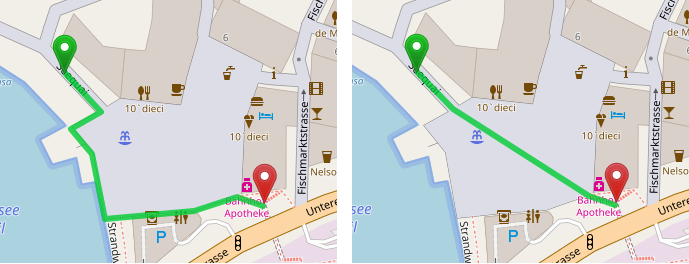
\includegraphics[width=1\linewidth]{technicalreport/img/compare_fischmarktplatz.png}
    \caption[Vergleich Ausgangslage und Ergebnis]{Vergleich aktueller Stand einer Routing-Engine (links) mit dem Ergebnis der Vorverarbeitung (rechts); Fischmarktplatz in Rapperswil, Schweiz; Screenshot aufgenommen am 17.12.17}
    \label{fig:compare_fischmarktplatz}
\end{figure}


\paragraph{Ziele, Vorgehen und Technologien}~\\
Im Kontext der Arbeit \emph{PlazaRoute} wird die Problematik des Fussgänger-Routings über offene Flächen im urbanen Raum aufgegriffen. Kurz zusammengefasst heisst das, dass eine Routing-Engine ein natürliches Fussgänger-Routing generieren kann.

In Kombination mit dem ÖV-Routing soll ein multimodales Routing möglich sein, welche Haltestellen genau ansteuert.

Um diese Anforderungen erfüllen zu können, werden Algorithmen zum Traversieren von offenen Fussgänger-Flächen evaluiert, analysiert, getestet und optimiert. Nach Abschluss dieser Tätigkeit wird es möglich sein, eine \ac{OSM} Datei so aufbereiten zu können, dass Routing-Engines dem Fussgänger ein natürliches Routing bieten können. Die durch die Algorithmen erzeugten Graphen werden mit Shortest-Path-Algorithmen vereinfacht, um die zusätzliche Datenmenge zu minimieren.
Um die Optimierung an einem praktischen Beispiel zeigen zu können, wird parallel in Kombination mit dem Service von search.ch ein ÖV-Routing entwickelt. Das multimodale Routing wird durch eine visuelle Darstellung in einem Plugin für das Geoinformationssystem QGIS abgerundet, welche den Mehrwert für einen Fussgänger konkret aufzeigen wird.

Die zugrundeliegende Technologie ist Python.

\paragraph{Ergebnisse}~\\
Durch die Umsetzung einer Vorverarbeitung mit einem Visibility-Graph oder SpiderWeb-Graph in Kombination mit einem Shortest-Path-Algorithmus (Dijkstra und A*) ist die Grundlage für ein natürliches Fussgänger-Routing geschaffen, auf welche gängige Routing-Engines und andere Interessenten operieren oder auf der Implementation aufsetzen können.

Fussgänger können zu jedem Zeitpunkt und auf jeder Position ein Routing durchführen, welches ihrem Verhalten entspricht.

\begin{figure}[ht]
    \centering
    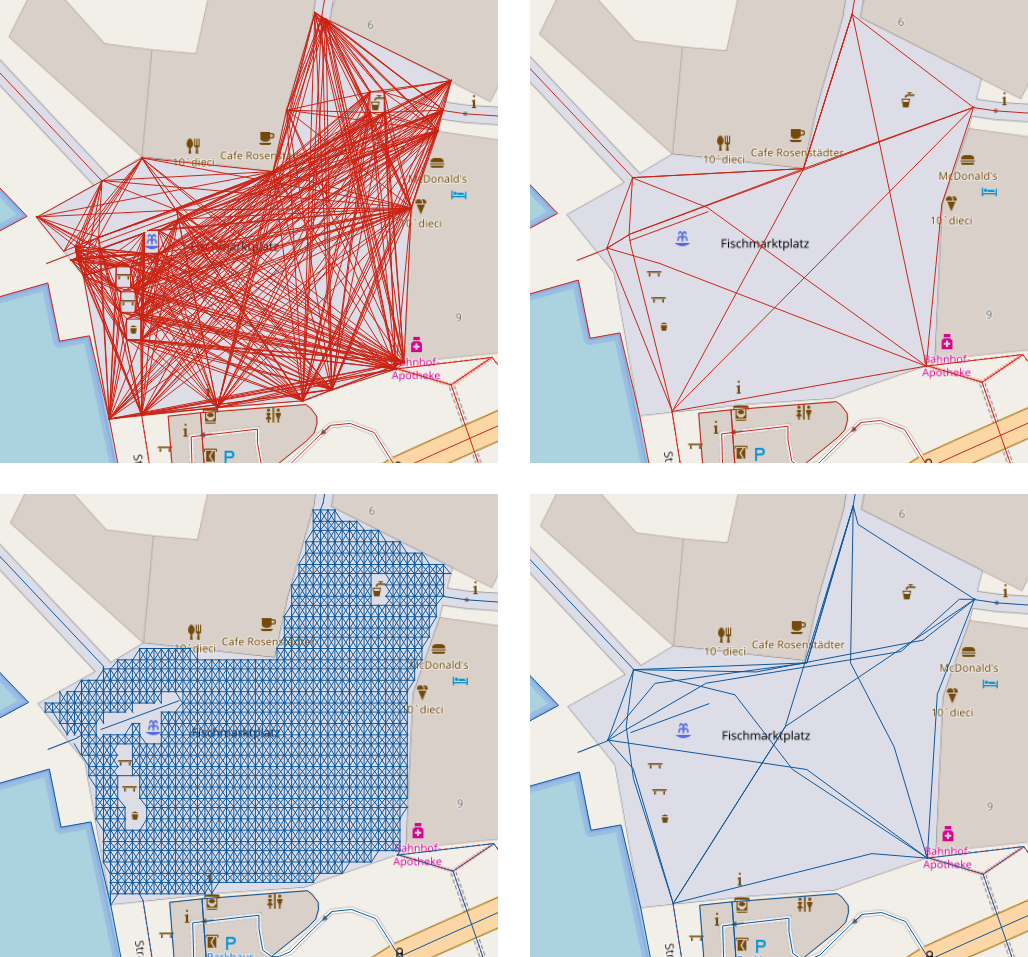
\includegraphics[width=0.8\linewidth]{technicalreport/img/proprecessing_optimization_comparison.png}
    \caption[Vergleich Preprocessing mit und ohne Optimierung]{Vergleich der Algorithmen Visibility-Graph (oben) und SpiderWeb-Graph (unten), vor und nach der Optimierung durch Shortest-Path-Algorithmen}
    \label{fig:proprecessing_optimization_comparison}
\end{figure}

Um bequem und auf direktem Weg nach Hause zu gelangen, ist das Transportmittel-übergreifende Routing als Service verfügbar und kann in einem QGIS-Plugin visualisiert werden.

\begin{figure}[ht]
    \centering
    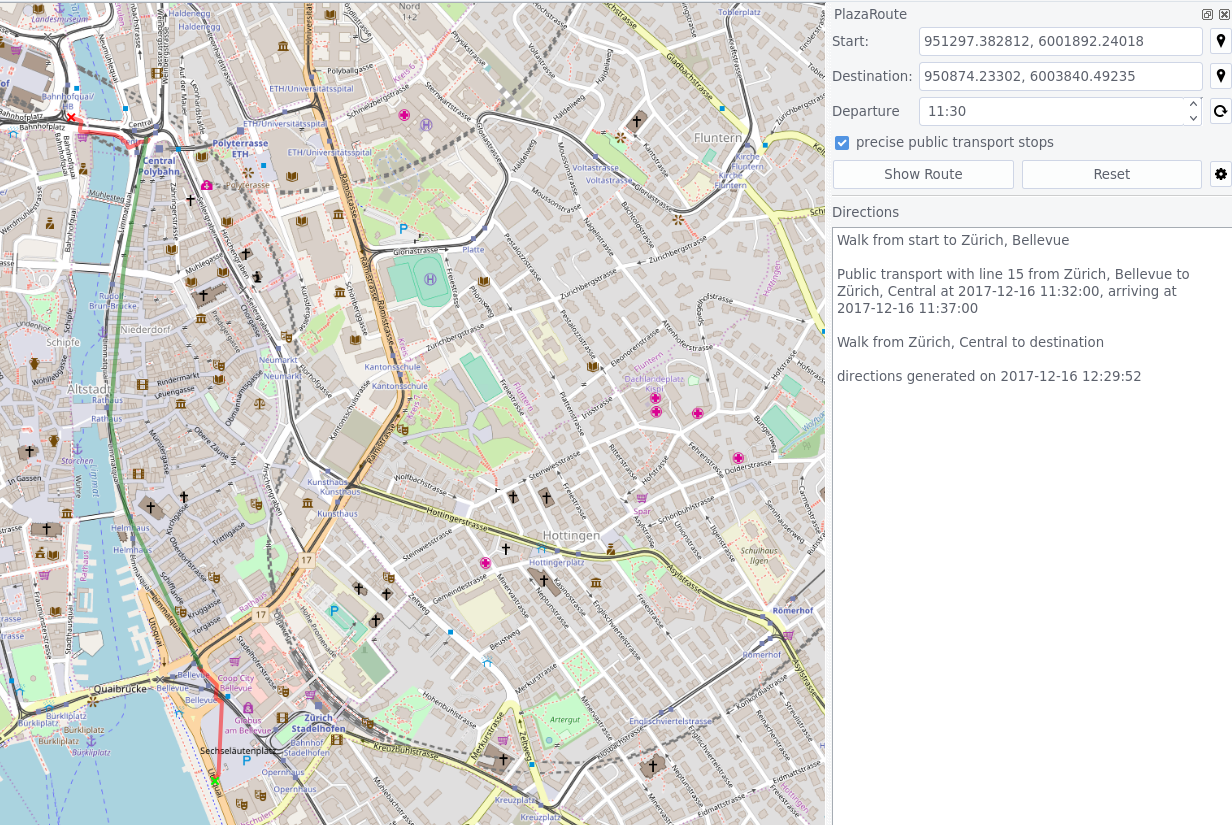
\includegraphics[width=1.0\linewidth]{technicalreport/img/qgis_plugin_plaza_route_cropped}
    \caption[Berechnete Route in QGIS-Plugin PlazaRoute]{Berechnete Route in QGIS-Plugin PlazaRoute}
    \label{fig:qgis_plugin_plaza_route_cropped}
\end{figure}

\paragraph{Ausblick}~\\
Die bestehende Lösung bietet weiteren Raum für Optimierungen. So können einige Plätze, welche für Fussgänger begehbar sind, durch fehlende \glspl{Einstiegspunkt} momentan nicht verarbeitet werden.

Die Arbeit hat sich bewusst auf den urbanen Raum beschränkt, da die Mehrheit der Routings in diesem Umfeld durchgeführt werden. Diese Grenze soll erweitert werden und Flächen ohne konkrete Begrenzungen wie Berge und Strände einbeziehen.

Die Vorverarbeitungen der Flächen stösst im Bezug auf die Performanz auf Grenzen. Ein Vergleich mit einer Lösung in PostGIS oder C++ ist denkbar.
